\subsection{Описание алгоритма GlobOpt}

Задача глобальной оптимизации состоит в поиске точки глобального минимума целевой функции $f: \mathbf{X} \rightarrow \mathbf{R}$ с помощью её интервального сужения $\mathbf{f}: \; \mathbb{IX} \rightarrow \mathbb{IR}$ с наперёд заданной точностью (шириной выходного интервала): $\textrm{wid} \; \mathbf{f(X^*)} < \varepsilon$.

Алгоритм \cite{globopt} работает по принципу половинного деления исходного бруса по некоторым координатам с записью пары ``(аргумент; значение'' в \textbf{рабочий список}. В наивной версии производятся все возможные половинные деления исходного бруса, однако достаточно рассекать только те, на которых достигаются нижний и верхний концы интервальной оценки области значений функции.

\subsection{Функция Растригина}
Функция задаётся следующим образом:
\begin{equation}
f_R = x^2 + y ^ 2 - \textrm{cos}(18x) - \textrm{cos}(18y)
\end{equation}
Достигает глобального минимума в точке $x^*={0;0}$. $f_R(x^*)=-2$.

\subsection{Функция Бута}
Функция задаётся следующим образом:
\begin{equation}
f(x, y) = (x + 2y - 7) ^ 2 + (2x + y - 5) ^ 2
\end{equation}

Достигает глобального минимума в точке $x^*={1;30}$. $f_R(x^*)=0$.

\begin{figure}[H]
	\begin{center}
		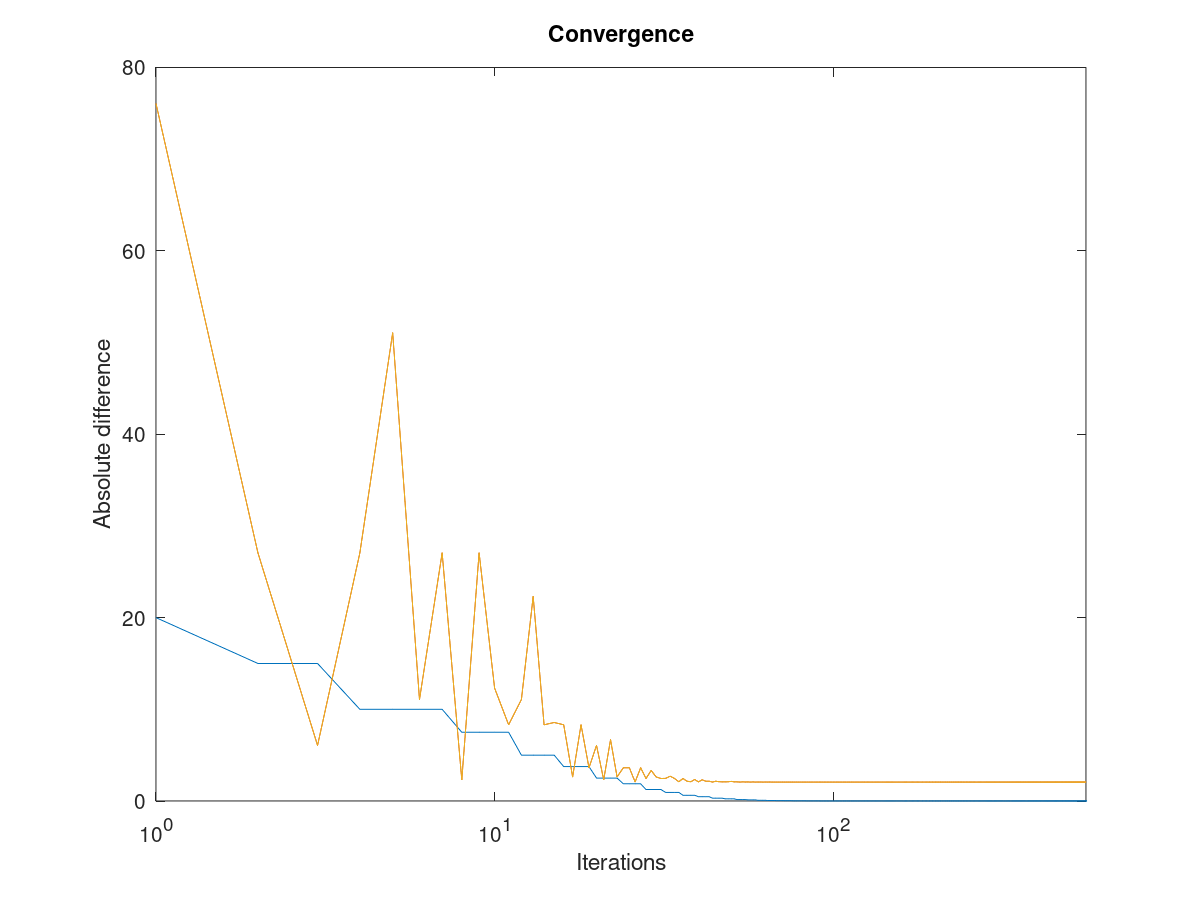
\includegraphics[scale=0.7]{booth}
		\label{pic:degenmat}
		\caption{Функция Бута}
	\end{center}
\end{figure}